\chapter{Desenvolvimento}
\lipsum[5-6]
\section{Fazendo Acontecer}
    Felis quam porttitor velit sodales ligula eget amet sociosqu iaculis, curabitur vel aptent curabitur ornare rutrum id sit, primis auctor tortor platea luctus sapien rutrum a. dui faucibus mi condimentum convallis non etiam placerat tristique fusce feugiat faucibus, praesent cubilia quisque mauris elit aenean etiam tellus pulvinar. curae aliquam morbi eros elementum feugiat pretium orci lobortis ac consectetur pharetra, ligula risus sagittis netus pellentesque suscipit quis viverra ac. aenean ornare senectus etiam leo auctor \cite{CARVALHOAMP:2012a} iaculis vulputate phasellus auctor, enim iaculis mauris tristique volutpat quisque justo amet vitae donec, vulputate donec cubilia feugiat rutrum congue sollicitudin semper. 

	Id cras quisque aliquam interdum malesuada volutpat senectus, proin justo varius etiam nisl at elit aliquet, donec viverra lacinia donec habitant et. accumsan curabitur viverra ultrices aliquam ut phasellus nisl, lorem lectus semper platea aliquam ut luctus, rhoncus eros quisque ipsum augue posuere. hendrerit torquent proin iaculis suspendisse placerat hendrerit viverra consequat, et ut suspendisse vestibulum hac curabitur tincidunt risus, sed dictum conubia senectus cras nulla scelerisque. nec enim nunc donec sagittis morbi mauris metus cubilia massa placerat quis facilisis dapibus congue, integer amet odio himenaeos nam non velit cras class rutrum semper senectus.
\section{Inserindo Tabelas}
\lipsum[7-8]
\subsection{Aqui Temos uma Tabela}
Uma singela tabelinha
\begin{table}[htb]
    \centering
    \caption{Singela Tabela}
    \label{tab:my-table}
    \begin{tabular}{c|c|c|c|}
    \cline{2-4}
     & \textbf{Coluna 01} & \textbf{Coluna 02} & \textbf{Coluna 03} \\ \hline
    \multicolumn{1}{|c|}{\textbf{Linha 01}} & 11 & 12 & 13 \\ \hline
    \multicolumn{1}{|c|}{\textbf{Linha 02}} & 21 & 22 & 23 \\ \hline
    \multicolumn{1}{|c|}{\textbf{Linha 03}} & 31 & 32 & 33 \\ \hline
    \end{tabular}
\end{table}
\subsection{Agora um Quadro}
\begin{quadro}[h]
    \centering
        \begin{tabular}{|c|c|c|c|}
            \hline 
            Aula & Conteúdo & Metodologia & Material Didático \\ 
            \hline 
            01 & CT01 & MT01 & MD01 \\ 
            \hline 
            02 & CT02 & MT02 & MD02 \\ 
            \hline 
            03 & CT03 & MT03 & MD04 \\ 
            \hline 
            04 & CT04 & MT04 & MD04 \\ 
            \hline 
            05 & CT05 & MT05 & MD05 \\ 
            \hline 
            06 & CT06 & MT06 & MD06 \\ 
            \hline 
        \end{tabular} 
        \caption{Quadro sintético de aulas}
        \label{qua:01}
    \end{quadro}
    \section{Equações}
    A fonte de campo magnético variável, ocorre devido à presença da corrente elétrica circundante nas espiras da bobina indutora, esta corrente elétrica sofre variações no sentido do fluxo a depender da frequência oscilante do circuito, para o caso, é escolhido valores de frequência suficientemente baixa a fim de desprezar-se os efeitos da corrente de deslocamento dada pela expressão $\partial D/\partial t$ na 4° Lei de Maxwell, conhecida como \emph{Lei de Ampère-Maxwell}. Neste caso, escreve-se as equações de Maxwell tal como:
\begin{align}	
	\begin{split}
		\label{eq:faraday}
		\vec{\nabla}\times\vec{E}&=-\parder{\vec{B}}{t},
	\end{split}
	\\
	\begin{split}
		\label{eq:ampere}		
		\vec{\nabla}\times\vec{H}&=\vec{J},
	\end{split}
	\\
	\begin{split}
		\label{eq:MagGauss}		
		\vec{\nabla}\cdot\vec{B}&=0.
	\end{split}
\end{align}
Considera-se ainda as condições de continuidade relacionadas entre os campos $\vec{B}$ e $\vec{H}$ assim como entre $\vec{J}$ e $\vec{E}$ descritas por:
\begin{align}
	\begin{split}
		\label{eq:contJ}
		\vec{\nabla}\times\vec{J}&=0,
	\end{split}
	\\
	\begin{split}
		\label{eq:conH}		
		\vec{B}&=\mu(\vec{r})\vec{H},
	\end{split}
	\\
	\begin{split}
		\label{eq:contE}		
		\vec{J}&=\sigma(\vec{r})\vec{E}.
	\end{split}
\end{align}
Por fim, o potencial vetor $\vec{A}$ é definido levando-se em conta a eq. \eqref{eq:MagGauss} como segue:
\begin{align}
	\label{eq:potVetor}
	\vec{\nabla}\times\vec{A}&=\vec{B}.
\end{align}
\section{Citações}
    Não se trata aqui de tornar o estagiário durante o exercício do estágio, um crítico contumaz à pratica docente observada em sala de aula, mas sim de fazê-lo 
\begin{citacao}
    ``[...]detectar e superar uma visão simplista dos problemas de ensino e aprendizagem, proporcionando dados significativos do cotidiano escolar que possibilitem uma \textbf{reflexão crítica} do trabalho a ser desenvolvido como professor e dos processos de ensino e aprendizagem em relação ao seu conteúdo específico.'' \cite[p. 11, \textbf{grifos meus}]{CARVALHOAMP:2012b} 
\end{citacao}
\section{Figuras}
\lipsum[8-9]
\subsection{Inserindo uma Figura}
A figura abaixo representa o fio próximo a massa $m$, um elemento de massa $dm$ é localizado na posição $x$
\begin{figure}[!h]
    \center
    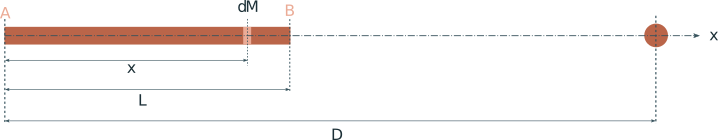
\includegraphics[scale=.7]{elementos/02-textual/fig/fio.png}
    \caption{Fio de dimensões não desprezíveis}
    \label{fig:1}
\end{figure}\\
A distância $d_1$ do ponto $A$ até a massa $m$ é $d_{1}=\vert D\vert$ e a distância $d_2$ do ponto $B$ até $M$ é $d_{2}=\vert D-L\vert$, dessa forma a média geométrica entre $d_1$ e $d_2$ é simplesmente
		\begin{align}
			d&=\sqrt{D(D-L)}.
			\label{eq:med-geo}
		\end{align}
O elemento de massa $dM$ ocupa um elemento de comprimento $dx$ do fio e sendo este fio homogêneo, vale a relação $\lambda=dM/dx$ ou ainda $\lambda=M/L$, além do mais $dM$ produz uma elemento de campo $d\vec{g}$ em $m$ tal que
		\begin{align}
			d\vec{g}&=-\frac{GdM}{(D-x)^2}\hat{i},
			\label{eq:eleme-g}
		\end{align}
onde o sinal em \eqref{eq:eleme-g} indica que a massa $m$ deve estar sob o efeito de uma força atrativa, característica do campo gravitacional. Substituindo $dM$ e integrando ao longo do fio tem-se
		\begin{align}
			\vec{g}=-\hat{i}G\lambda\int_{0}^{L}\frac{dx}{(D-x)^2},
			\label{eq:int1}
		\end{align}
fazendo $u=D-x$ então $du=-dx$, resolvendo integral pelo método da substituição chega-se em
		\begin{align}
			\vec{g}&=-\hat{i}\lambda G\left(\frac{1}{D-L}-\frac{1}{D}\right)\nonumber\\
				   &=-\hat{i}\lambda G\left[\frac{L}{D(D-L)}\right],
		\label{eq:final1}
		\end{align}
substituindo $\lambda$ e notando que em \eqref{eq:med-geo} $d^{2}=D(D-L)$ a eq. \eqref{eq:final1} torna-se
		\begin{align}
			\vec{g}&=-\frac{MG}{L}\left(\frac{L}{d^2}\right)\hat{i}
		\end{align}
por fim temos
		\begin{align}
			\vec{g}&=-\frac{GM}{d^2}\hat{i},
		\end{align}
semelhante à forma do campo gravitacional a uma distância $d$ da massa pontual $M$, geradora do campo.
    